\documentclass{amsart}
\usepackage{amsmath,amssymb,amsthm,amsfonts,amscd,mathrsfs,mathtools}
\usepackage{graphicx}
\usepackage[hyphens]{url}
\usepackage{caption}
\usepackage{hyperref}



\theoremstyle{plain}
    \newtheorem{thm}{Theorem}[section]
    \newtheorem{lem}[thm]   {Lemma}
    \newtheorem{cor}[thm]   {Corollary}

\theoremstyle{definition}
    \newtheorem{defn}[thm]  {Definition}
    \newtheorem{conj}[thm]{Conjecture}

\newcommand{\C}{\mathbb{C}}
\newcommand{\cC}{\mathfrak{C}}
\newcommand{\fc}{\mathfrak{c}}
\newcommand{\D}{\mathcal{D}}
\newcommand{\F}{\mathbb{F}}
\newcommand{\cF}{\mathcal{F}}
\renewcommand{\H}{\mathcal{H}}
\newcommand{\M}{\mathcal{M}}
\newcommand{\N}{\mathcal{N}}
\newcommand{\p}{p}
\newcommand{\cP}{\mathcal{P}}
\newcommand{\Q}{\mathbb{Q}}
\newcommand{\R}{\mathbb{R}}
\renewcommand{\S}{\mathcal{S}}
\newcommand{\fS}{\mathfrak{S}}
\newcommand{\T}{\mathcal{T}}
\newcommand{\U}{\mathcal{U}}
\renewcommand{\u}{\mathfrak{u}}
\newcommand{\V}{\mathcal{V}}
\renewcommand{\v}{\mathfrak{v}}

\newcommand{\Z}{\mathbb{Z}}


\newcommand{\sgm}{\Sigma_{g,1}^m}
\newcommand{\sg}{\Sigma_{g,1}}

\newcommand{\Sg}{\mathcal{S}_{g,1}}
\newcommand{\Sgm}{\Sg^m}

\newcommand{\mg}{\mathfrak{M}_{g,1}}
\newcommand{\mgm}{\mg^m}
\newcommand{\Ig}{\mathcal{I}_{g,1}}

\renewcommand{\gg}{\Gamma_{g,1}}
\newcommand{\ggm}{\gg^m}

\newcommand{\bms}{\beta_{m}(\sg)}
\newcommand{\fms}{F_m(\sg)}
\newcommand{\cms}{C_m(\S)}
\newcommand{\fmsD}{C_{1,m}^{\D}(\S)}
\newcommand{\cmsD}{C_{m}^{\D}(\S)}
\newcommand{\fmstwoD}{C_{1,m}^{(2),\D}(\S)}
\newcommand{\cmstwoD}{C_{m+1}^{(2),\D}(\S)}
\newcommand{\Dmone}{\triangle_{m+1}}
\newcommand{\Donem}{\triangle_{1,m}}
\renewcommand{\i}{\iota}
\renewcommand{\j}{j}
\newcommand{\pr}{\mathfrak{p}}

\newcommand{\symb}{\mathcal{S}}
\newcommand{\bsymb}{\bar\symb}
\newcommand{\tup}{\mathfrak{h}}

\newcommand{\bH}{\mathbb{H}}
\newcommand{\cH}{\mathcal{H}}

\newcommand{\Ch}{\mathcal{C}}
\newcommand{\tCh}{\tilde\Ch}
\newcommand{\tH}{\tilde{H}}

\newcommand{\ZcC}[1]{\Z_2\left<\cC^{#1}\right>}
\newcommand{\tpsi}{\tilde\psi}

\newcommand{\pa}[1]{\left(#1\right)}
\newcommand{\qua}[1]{\left[#1\right]}
\newcommand{\abs}[1]{\left|#1\right|}
\newcommand{\set}[1]{\left\{#1\right\}}

\newcommand{\Sone}{\mathbb{S}^1}
\newcommand{\mrS}{\mathring{\S}}
\newcommand{\gone}{\Gamma_{1,1}}
\newcommand{\tu}{\tau_{\u}}
\newcommand{\tv}{\tau_{\v}}

\newcommand{\ux}{\underline{x}}
\newcommand{\uu}{\underline{u}}
\newcommand{\uv}{\underline{v}}
\newcommand{\ualpha}{\underline{\alpha}}

\newcommand{\tildeu}{\tilde u}
\newcommand{\tildev}{\tilde v}

\newcommand{\SP}{S\!P}

\renewcommand{\phi}{\varphi}
\renewcommand{\epsilon}{\varepsilon}

\newcommand{\hor}{hor}
\newcommand{\ver}{ver}

\renewcommand{\L}{\Lambda}
\DeclareMathOperator{\Diff}{Diff}
\DeclareMathOperator{\Imm}{Imm}
\DeclareMathOperator{\rk}{rk}
\DeclareMathOperator{\Ker}{ker}
\DeclareMathOperator{\coker}{coker}
\DeclareMathOperator{\Sym}{Sym}
\DeclareMathOperator{\Id}{Id}
\DeclareMathOperator{\Hom}{Hom}


\DeclarePairedDelimiter\ceil{\lceil}{\rceil}
\DeclarePairedDelimiter\floor{\lfloor}{\rfloor}
\def\colim{\mathop{\mathrm{colim}}\nolimits}
    
\begin{document}

\title{Splitting of the homology of the punctured mapping class group}

\author{Andrea Bianchi}

\address{Mathematics Institute,
University of Bonn,
Endenicher Allee 60, Bonn,
Germany
}



\email{bianchi@math.uni-bonn.de}

\date{\today}


%\keywords{Topological complexity, aspherical spaces, Lusternik-Schnirelmann category, cohomological dimension, topological robotics, braid groups}
%\subjclass[2010]{55M99, 55P20 (Primary); 55M30, 20J06, 68T40 (Secondary).}

\begin{abstract}
Let $\ggm$ be the mapping class group of an orientable surface $\sgm$ of genus $g$ with one parametrised
boundary component and $m$ permutable punctures, and let $\bms$ be the braid group on $m$ strands
of the surface $\sg$. We prove that $H_*(\ggm;\Z_2)\cong H_*(\gg;H_*(\bms;\Z_2))$.
We compute (?) the right hand side explicitly for $g=1$.
\end{abstract}

%\thanks{}

\maketitle

\section{Introduction}
Let $\sg$ be a smooth orientable surface of genus $g$ with one boundary curve $\partial\sg$, and let $\sgm$ be $\sg$ with
a choice of $m$ distinct points in the interior, called \emph{punctures}.

Let $\gg$ be the mapping class group of $\sg$, i.e. the group of isotopy classes of diffeomorphisms of $\sg$:
diffeomorphisms are required to fix $\partial\sg$ pointwise. Similarly let $\ggm$ be the mapping class group of $\sgm$, i.e.
the group of isotopy classes of diffeomorphisms of $\sgm$ that fix $\partial\sgm$ pointwise and \emph{permute} the $m$ punctures.

Forgetting the punctures gives a surjective map $\ggm\to\gg$ with kernel $\bms$,
the $m$-th \emph{braid group} of the surface $\sg$. We obtain the Birman exact sequence (see \cite{Birman:mcgbr})
\begin{equation}
\label{eq:Birman}
1\to\bms\to\ggm\to\gg\to 1.
\end{equation}
% This short exact sequence corresponds to 
% \begin{equation}
%  \cms\to\mgm\to\mg.
% \end{equation}
% Here $\cms$ is the \emph{unordered} configuration space of $m$ points in the interior of $\Sigma$, i.e.
% \begin{equation}
%  \cms=\fms/\S_m=\set{(p_1,\dots,p_m)\in\pa{\mathring\sg}^m|p_i\neq p_j \;\forall i\neq j}/\S_m,
% \end{equation}
% the quotient of the \emph{ordered} configuration space of $m$ points in the interior of $\Sigma$ by the natural
% action of the symmetric group $\S_m$ that permutes the (ordered list of) points in the configuration; $\mg$ and $\mgm$
% are the moduli spaces of Riemann structures on $\sg$ and $\sgm$ respectively.

The associated Leray-Serre spectral sequence $E(m)$ in $\Z_2$-homology has a second page $E(m)^2_{k,q}=H_k(\gg;H_q(\bms;\Z_2))$,
and converges to $H_{k+q}(\ggm;\Z_2)$.

The main result of this article is that this spectral sequence collapses in its second page.
\begin{thm}
\label{thm:main}
For all $l\geq 0$ there is an isomorphism of vector spaces
\begin{equation}
\label{eq:main}
H_l\pa{\ggm;\Z_2}\cong \bigoplus_{k+q=l} H_k\pa{\gg;H_q\pa{\bms;\Z_2}}.
\end{equation}
\end{thm}
Thus the computation of $H_*\pa{\ggm;\Z_2}$ reduces to the computation of the homology of $\gg$ with
twisted coefficients in the representation $H_*\pa{\bms;\Z_2}$. We will see that this $\gg$-representation
splits as a direct sum of symmetric powers of $H_1(\sg)$ with the symplectic action: this is done in
Theorem \ref{thm:Hbms*as*ggrep}, which together with Theorem \ref{thm:main} is the main result of the article.
% in section \ref{sec:HBraidSurf}).

%In particular this representation is symplectic: this had already benn stated in \cite{LM}.

% The group $\gg$ is significantly smaller than $\ggm$, so the
% computation of the right-hand side of equation \eqref{eq:main}
% may be more tractable.
%WE DO THIS COMPUTATION FOR $g=1$.

The strategy of the proof does not generalize to fields of characteristic different from 2 or to the \emph{pure}
mapping class group, in which we consider only diffeomorphisms of $\sgm$ that fix all punctures. In section \ref{sec:rational}
we describe in detail a counterexample with coefficients in $\Q$, which can be generalized both to coefficients
in a field $\F_p$ of odd characteristic and to the pure mapping class group.

I would like to thank my PhD advisor Carl-Friedrich B\"odigheimer for his precious suggestions and his continuous encouragement
during the preparation of this work.

\section{Preliminaries}
\label{sec:Preliminaries}
In the whole article $\Z_2$-coefficients for homology and cohomology will be understood,
unless explicitly stated otherwise.

In this section we recollect some classical definitions and results about braid groups and mapping class groups.
Let $\sg$ be a compact, smooth, orientable surface of genus $g$ with one parametrised
boundary component $\partial \sg$. Let $\sgm$ be $\sg$ with a choice of $m$ distinct
points in the interior: these points are called \emph{punctures} and are not assumed to be ordered.

\begin{defn}
\label{defn:cms}
 The $m$-th \emph{ordered configuration space} of a surface $\sg$ is the space
\[
 F_m(\sg)=\set{(P_1,\dots,P_m) \in \pa{\mathring{\Sigma}_{g,1}}^{\times m}  \,|\,  P_i\neq P_j  \;\forall i\neq j}.
\]

 Notice that we require the points of the configuration to lie in the interior of $\sg$;
 $F_m(\sg)$ is a smooth, orientable $2m-$dimensional manifold.
 
 The symmetric group $\mathfrak{S}_m$ acts freely on $F_m(\sg)$ by permuting the points of a configuration;
 the orbit space
 \[
 F_m(\sg)/\mathfrak{S}_m
 \]
 is called the \emph{$m-$th unordered configuration space}
 of $\sg$ and is denoted by $C_m(\sg)$; this space is also a $2m-$dimensional orientable manifold
 (see figure \ref{fig:unordered}).
 
%  
%  We denote by $C_k(\sg)^c$ the one-point compactification of the space $C_k(\sg)$; the point
%  at infinity is denoted by $*$ and serves as basepoint.
\end{defn}

\begin{figure}\centering
 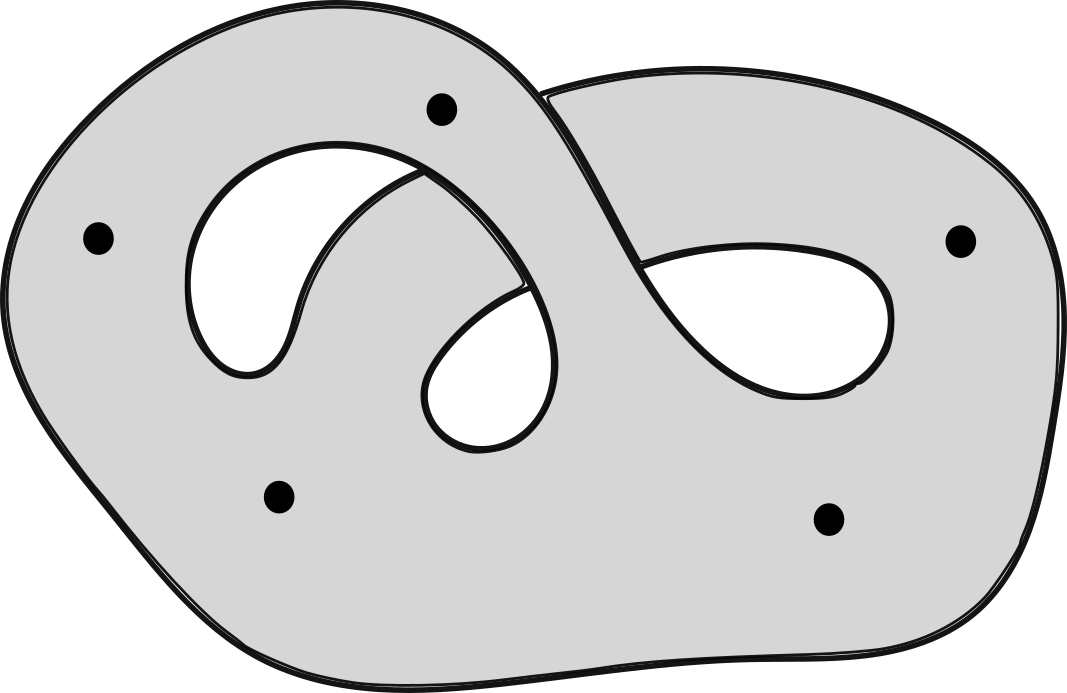
\includegraphics[scale=0.8]{figures/unordered.png}
 \caption{A configuration in the space $C_5(\Sigma_{1,1})$}
\label{fig:unordered}
\end{figure}


A classical result by Fadell and Neuwirth (\cite{FadellNeuwirth}) ensures
that $C_m(\sg)$ is aspherical; the fundamental group $\pi_1(C_m(\sg))$ is
called the \emph{braid group on $m$ strands of $\sg$} and is denoted by $\bms$.

\begin{defn}
 \label{def:mcg}
 Let $\Diff(\sg;\partial\sg)$ be the group of diffeomorphisms of $\sg$ that fix $\partial\sg$ pointwise,
 endowed with the Whitney $C^{\infty}-$topology. We denote by $\gg=\pi_0(\Diff(\sg;\partial\sg))$ its group of connected
 components, which is called the \emph{mapping class group} of $\sg$.
 
 Similarly let $\Diff(\sgm;\partial\sgm)$ be the group of diffeomorphisms of $\sgm$ that fix $\partial(\sg)$
 pointwise and restrict to a permutation of the $m$ punctures, and let $\ggm=\pi_0(\Diff(\sgm;\partial\sgm))$ be its
 group of connected components, called the mapping class group of $\sgm$.
 \end{defn}
 A classical result by Earle and Schatz (\cite{EarleSchatz}) ensures that the connected components
 of $\Diff(\sg)$ are contractible. In particular $B\Diff(\sg;\partial\sg)\simeq B\gg$ is
 a classifying space for
 the group $\gg$, i.e. a space of type $K(\gg,1)$; we call $\cF_{g,1}\to B\Diff(\sg;\partial\sg)$ the universal
 $\sg-$bundle
 \[
  \cF_{g,1}\colon=\sg\times_{\Diff(\sg;\partial\sg)}E\Diff(\sg;\partial\sg)\to B\Diff(\sg;\partial\sg).
 \]
Applying the construction of the $m-$th unordered configuration space fiberwise we obtain a bundle
$C_m(\cF_{g,1})\to B\Diff(\sg;\partial\sg)$ with fiber $C_m(\sg)$.

The space $C_m(\cF_{g,1})$ is a classifying space for the
group $\ggm$ and the Birman exact sequence \ref{eq:Birman} is obtained by taking fundamental
groups of the aspherical spaces
\begin{equation}\label{eq:Birmanbundle}
C_m(\sg)\to C_m(\cF_{g,1})\to B\Diff(\sg;\partial\sg).
\end{equation}

In the whole article the genus $g$ of the surfaces that we consider is supposed to be fixed,
unless explicitly stated otherwise, and we will abbreviate $\S=\sg$.
We denote by $\D$ the open disc $\mathring{\Sigma}_{0,1}$.

It will be useful, for many constructions, to choose an embedding
$\D\hookrightarrow\mrS$ near $\partial\S$ and to replace
$\Diff(\S;\partial\S)$ with its subgroup $\Diff(\S;\partial\S\cup\D)$ of diffeomorphisms
of $\S$ that fix pointwise both $\partial\S$ and $\D$. Saying that $\D$ is embedded
\emph{near $\partial\S$} means that there is a compact subsurface $\S'\subset\S$
such that $\S$ is the boundary connected sum $\S'\natural\bar\D$.
From now on we suppose such an embedding to be fixed and we consider $\D$ as a subspace
of $\mrS$ (see figure \ref{fig:SS'D}). In section \ref{sec:HBraidSurf}, definition \ref{defn:Tsg},
we will specify an embedding $\D\hookrightarrow\mrS$ using a particular model for $\mrS$.

\begin{figure}\centering
 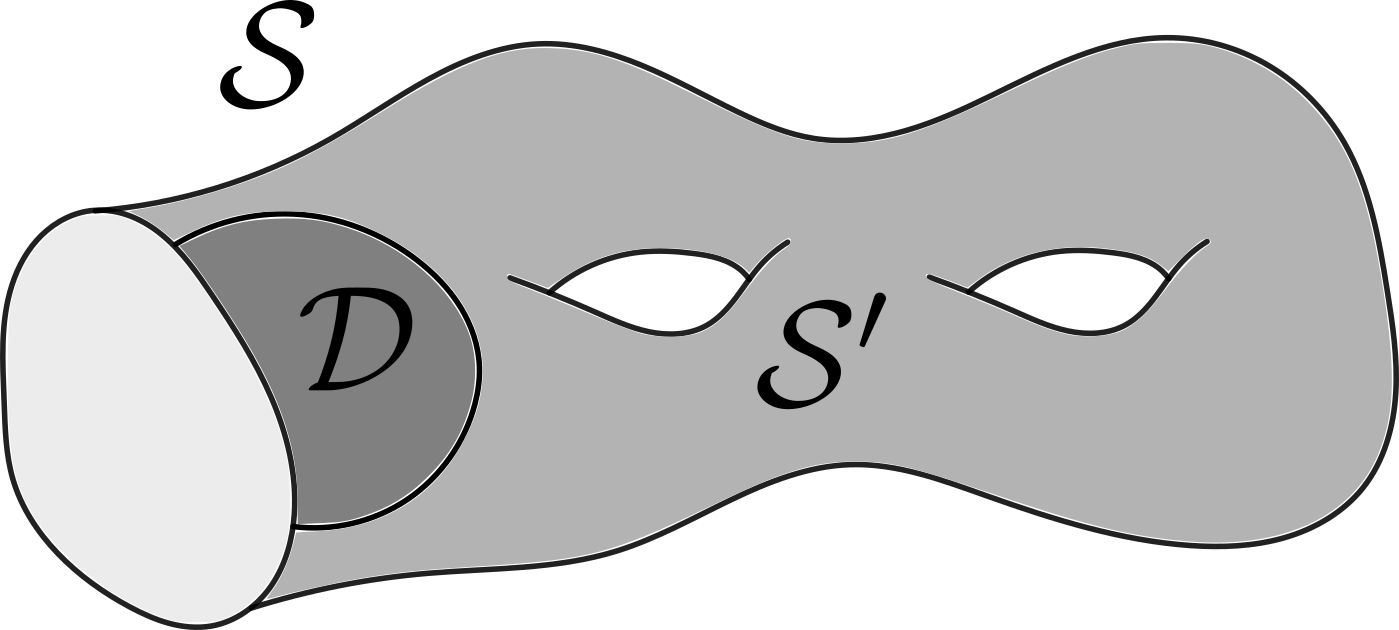
\includegraphics[scale=0.8]{figures/SS'D.png}
 \caption{A splitting of $\S$ as $\S'\natural\bar\D$.}
\label{fig:SS'D}
\end{figure}

The construction of definition \ref{defn:cms} can be specialised to the
surfaces $\D$ and $\S'$, yielding spaces $C_m(\D)$ and $C_m(\S')$ respectively.

The inclusion $\Diff(\S;\partial\S\cup\D)\subset\Diff(\S;\partial\S)$ is a homotopy
equivalence, hence also the induced map
\[
B\Diff(\S;\partial\S\cup\D)\to B\Diff(\S;\partial\S)
\]
is a homotopy equivalence. We will replace the previous construction with the following,
equivalent ones.
\begin{defn}
\label{defn:universalSbundle}
We call $\cF_{\S,\D}\to B\Diff(\S;\partial\S\cup\D)$
the universal $\S-$bundle
 \[
  \cF_{\S,\D}\colon=\S\times_{\Diff(\S;\partial\S\cup\D)}E\Diff(\S;\partial\S\cup\D)\to B\Diff(\S;\partial\S\cup\D).
 \]
Notice that $\Diff(\S;\partial\S\cup\D)$ acts on $\S'$ by restriction of diffeomorphisms, and acts trivially
on $\D$; therefore $\cF_{\S,\D}$ contains subspaces
\[
 \cF_{\S'}= \S'\times_{\Diff(\S;\partial\S\cup\D)}E\Diff(\S;\partial\S\cup\D)
\]
and $\D\times B\Diff(\S;\partial\S\cup\D)$; these subspaces fiber over $B\Diff(\S;\partial\S\cup\D)$
with fibers $\S'$ and $\D$ respectively.

Applying the construction of the $m-$th unordered configuration space fiberwise, we obtain spaces
$C_m(\cF_{\S,\D})$, $C_m(\cF_{\S'})$ and $C_m(\D)\times B\Diff(\S;\partial\S\cup\D)$,
all fibering over $B\Diff(\S;\partial\S\cup\D)$ with fibers, respectively, $\cms$,
$C_m(\S')$ and $C_m(\D)$.
\end{defn}

\begin{defn}
For all $0\leq p\leq m$ there is a natural map
\[
 \mu\colon C_p(\D)\times C_{m-p}(\S')\to \cms
\]
which takes the union of configurations (see figure \ref{fig:defmu}):
 \[
  \mu\pa{\set{P_1,\dots,P_p};\set{P'_1,\dots,P'_{m-p}}}=\set{P_1,\dots,P_p,P'_1,\dots,P'_{m-p}}\in\cms.
 \]
\begin{figure}\centering
 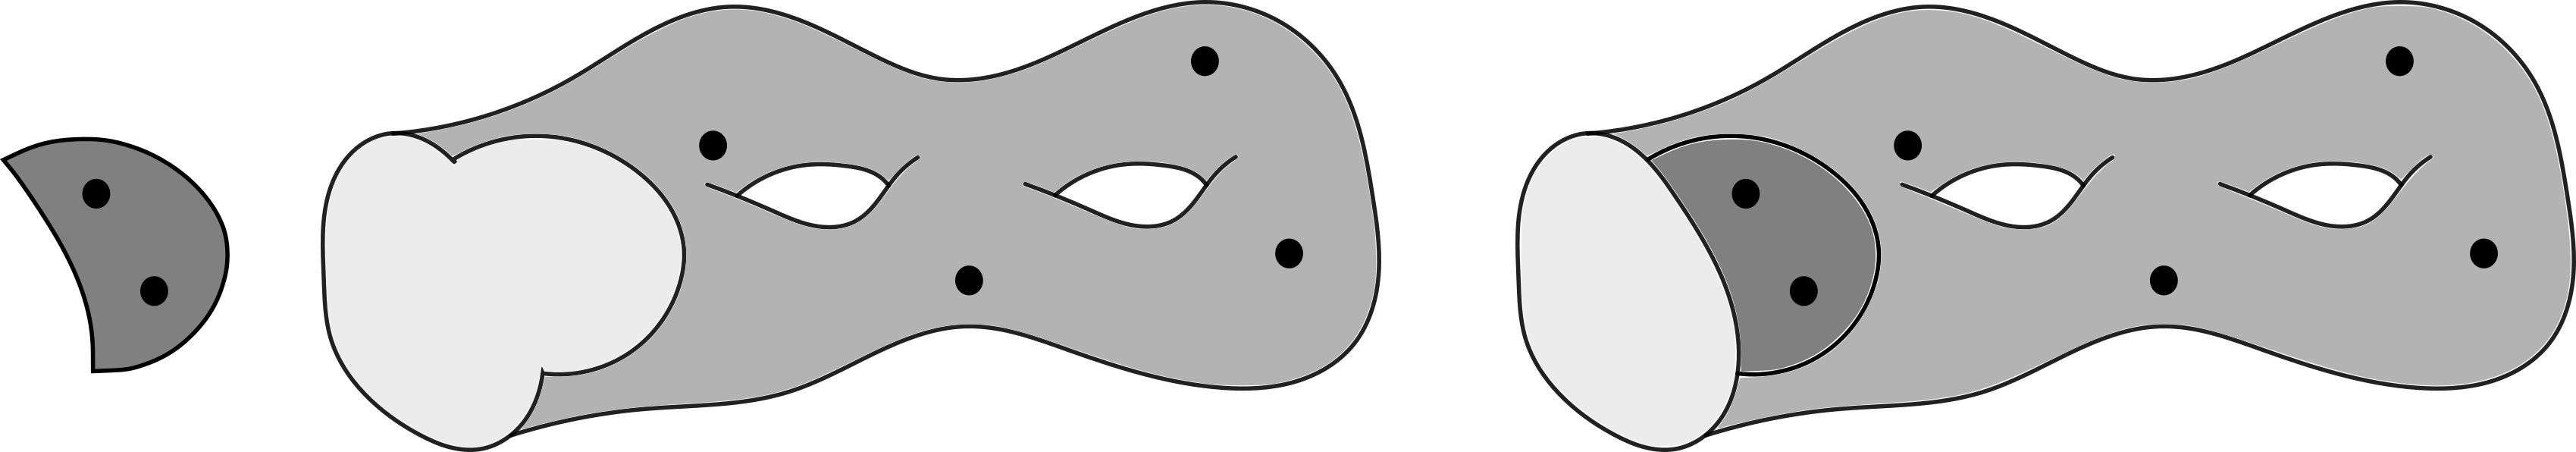
\includegraphics[scale=0.7]{figures/defmu.png}
 \caption{The product of two configurations in $C_2(\D)$ and $C_4(\S)$.}
\label{fig:defmu}
\end{figure}
 
We can apply this construction to each couple of fibers of $C_m(\cF_{\S,\D})$ and $C_{m-p}(\cF_{\S'})$
over the same point of $ B\Diff(\S;\partial\S\cup\D)$, obtaining a map $\mu^{\cF}$:
\[
 \mu^{\cF}\colon C_p(\D)\times C_{m-p}(\cF_{\S'})\to C_m(\cF_{\S,\D}).
\]
If we see the domain of $\mu^{\cF}$ as a fibered product of bundles over $B\Diff(\S;\partial\S\cup\D)$
\[
 \pa{C_m(\D)\times B\Diff(\S;\partial\S\cup\D)}\times_{B\Diff(\S;\partial\S\cup\D)}C_{m-p}(\cF_{\S'}),
\]
then the map $\mu^{\cF}$ is also a map of bundles over $B\Diff(\S;\partial\S\cup\D)$, and the corresponding
map on fibers is precisely $\mu$.
\end{defn}
The fiber bundle \ref{eq:Birmanbundle} corresponding to the Birman exact sequence \ref{eq:Birman}
can now be replaced by the following one
\begin{equation}\label{eq:BirmanbundleD}
\cms\to C_m(\cF_{\S,\D})\to B\Diff(\S;\partial\S\cup\D).
\end{equation}
We conclude this section by recalling the structure of $H_*(C_m(\D))$.

The cohomology of $C_m(\D)$ with coefficients in $\Z_2$ was first computed by Fuchs in
\cite{Fuchs:CohomBraidModtwo}: we will recall this computation in section
\ref{sec:HBraidSurf}, where we will make a similar computation in detail.

In \cite[Chap.III]{CLM} Cohen considers the space $\coprod_{m\geq 0}C_m(\D)$ as an
algebra over the operad of little $2-$cubes, and describes its
$\Z_2-$homology as follows:
\begin{equation}
 \label{eq:Cohen}
H_*\pa{\coprod_{m\geq 0}C_m(\D)}\simeq \Z_2\left[Q^j\epsilon \, |\, j\geq 0\right].
\end{equation}

Here $\epsilon\in H_0(C_1(\D))$ is the fundamental class, and for all
$k,m\geq 0$ we denote by $Q\colon H_k(C_m(\D))\to H_{2k+1}(C_{2m}(\D))$
the first Dyer-Lashof operation. In particular $Q^j\epsilon$ is the generator of
$H_{2^j-1}(C_{2^j}(\D))\simeq\Z_2$. See figure \ref{fig:monomial}

The isomorphism in equation \ref{eq:Cohen} is
an isomorphism of bigraded rings. The left-hand side is a ring with the Pontryagin product
coming from the action of the little $2-$cubes,
and the right-hand side is a polynomial ring in infinitely many variables $\epsilon,Q\epsilon,Q^2\epsilon,\dots$.
The bidegree is given by the homological degree
$*$, that we simply call the \emph{degree},
and by the index $m$ of the connected component
on which the homology class is supported (informally, the number of points
involved in the construction of a homology class), that we call the \emph{weight}.

 \begin{figure}\centering
 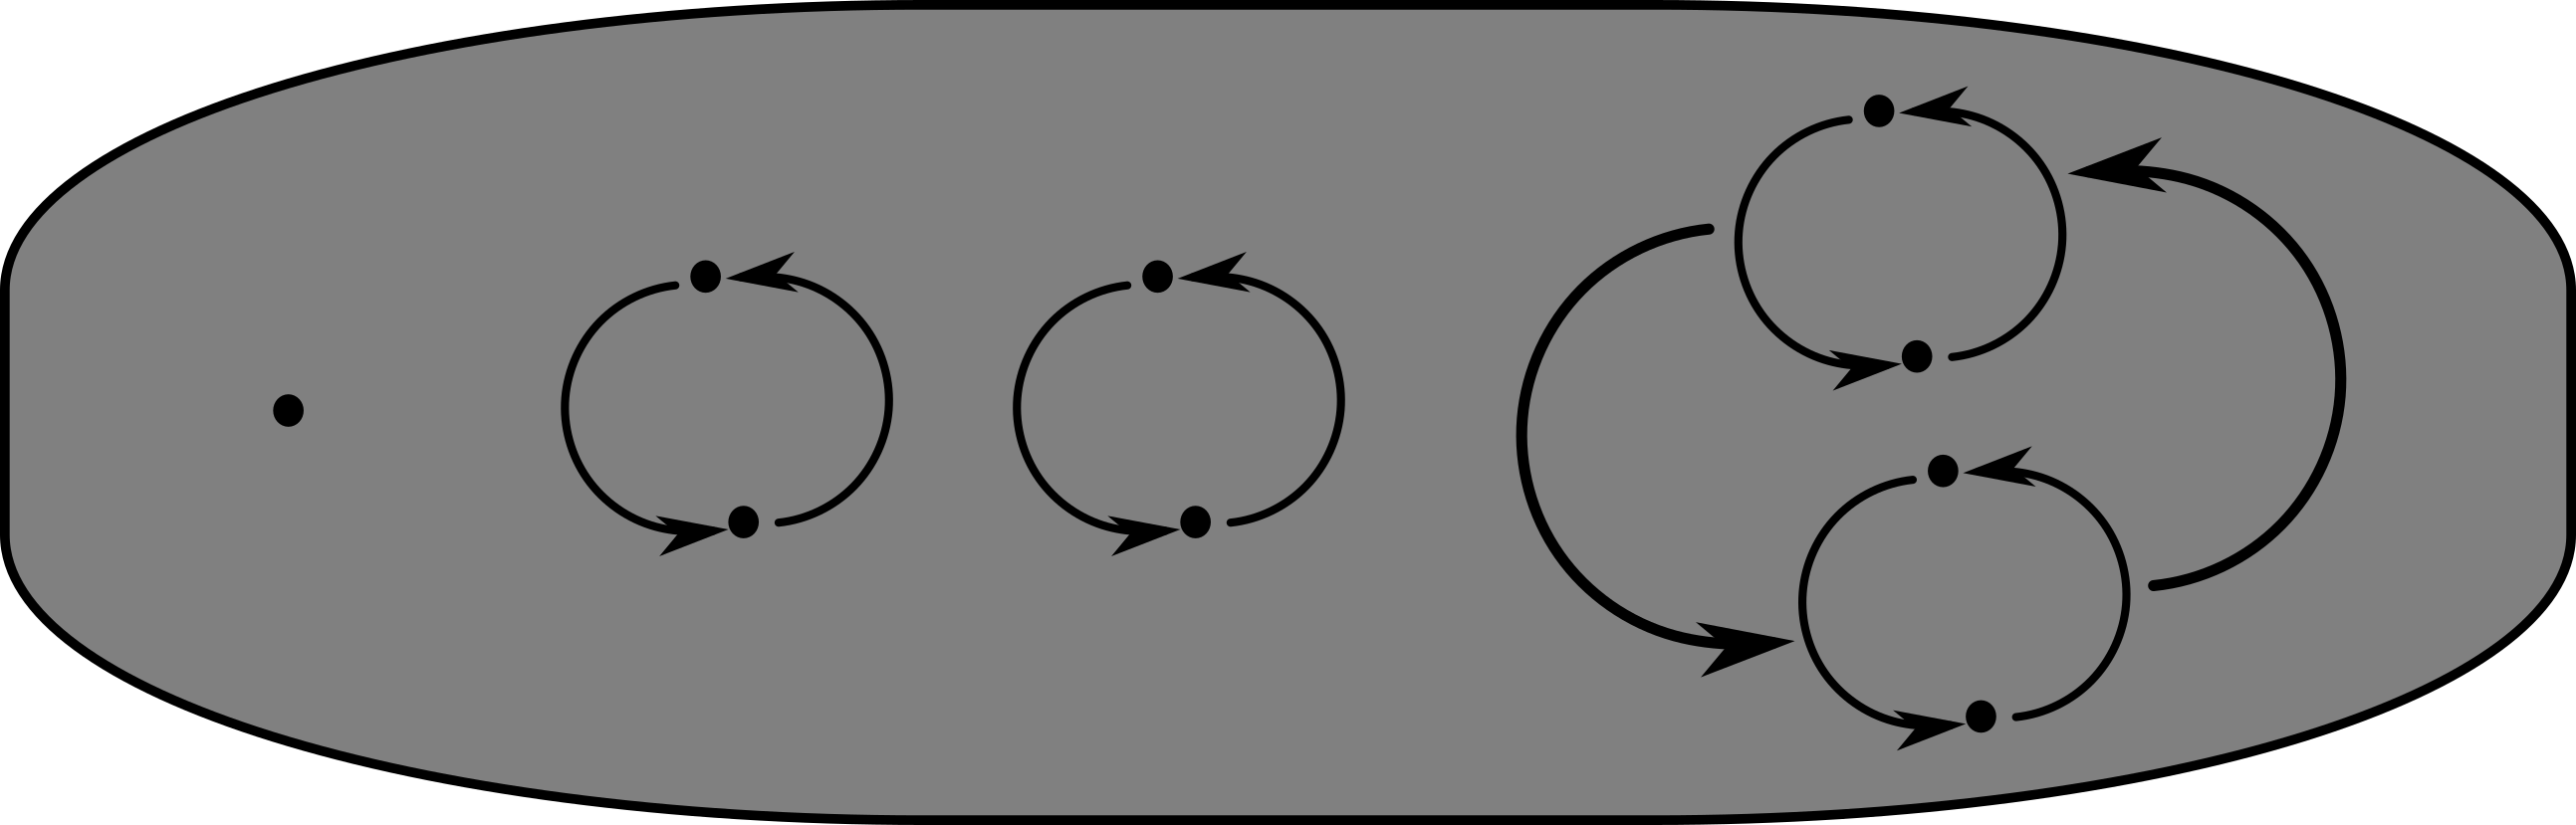
\includegraphics[scale=0.7]{figures/monomial.png}
 \caption{The class in $H_5(C_9(\D))$ corresponding to the monomial $\epsilon\cdot(Q\epsilon)^2\cdot Q^2\epsilon$.}
\label{fig:monomial}
\end{figure}

In this article we will only need the isomorphism in equation \ref{eq:Cohen} to hold as
an isomorphism of bigraded $\Z_2-$vector spaces.
In particular for all choices of natural numbers $(\alpha_j)_{j\geq 0}$ with all but finitely
many $\alpha_j=0$, we will consider the monomial $\prod_j\pa{Q^j\epsilon}^{\alpha_j}$, corresponding to
a homology class in some bidegree $(*,m)$: all that
we are going to need is that the set of these monomials is a bigraded basis for the
left-hand side of equation \ref{eq:Cohen}.

\section{Homology of configuration spaces of surfaces}
\label{sec:HBraidSurf}
We want to understand the homology groups $H_*(\bms)=H_*(C_m(\sg))$: we
are interested in these groups as they appear as the homology of the fiber
in the Leray-Serre spectral sequence associated to
\ref{eq:Birman}, \ref{eq:Birmanbundle} or \ref{eq:BirmanbundleD}.
In particular we are interested in $H_*(C_m(\S))$
as a $\Z_2-$representation of the group $\gg$.

In \cite{LM} L\"offler and Milgram proved that this must be a $\Z_2-$symplectic
representation of the mapping class group. By \emph{$\Z_2-$symplectic} we mean the following:
\begin{defn}
 \label{defn:symplrep}
 Let $\H=H_1(\S)\simeq\Z_2^{2g}$.
 The natural action of $\gg$ on $\H$ induces a surjective map
 $\gg\to Sp_{2g}(\Z_2)$. A representation of $\gg$ over $\Z_2$ is called \emph{$\Z_2-$symplectic}
 if it is a pull-back of a representation of $Sp_{2g}(\Z_2)$ along this map.
\end{defn}

In \cite{BCT} B\"odigheimer, Cohen and Taylor computed $H_*(C_m(\sg))$ \emph{as a graded $\Z_2-$vector space}.
Their method provides all Betti numbers, but the action of $\gg$ cannot be easily deduced, as
their descripition of $H_*(C_m(\sg))$ depends on a handle decomposition of $\sg$, which is not preserved,
not even up to isotopy, by diffeomorphisms of $\sg$.

In this section and in the next one we will prove the following theorem; to the best of the author's knowledge
it doesn't appear in the literature.
\begin{thm}
 \label{thm:Hbms*as*ggrep}
 There is an isomorphism of bigraded $\Z_2-$representations of $\gg$
 \[
  \bigoplus_{m\geq 0} H_*\pa{C_m(\sg)}\simeq \Z_2\left[Q^j\epsilon\,|\, j\geq 0\right]\otimes\Sym_{\bullet}(\H).
 \]
 Here we mean the following:
 \begin{itemize}
  \item the bidegree is given on left by homological degree $*$ and by the direct summand,
  indexed by $m$,
  on which the homology class is supported, i.e. by the number $m$ of points
  involved in constructing the homology class; we call $*$ the \emph{degree} and $m$ the \emph{weight},
  and write $(*,m)$ for the bidegree;
  \item for $j\geq 0$, $Q^j\epsilon$ is the image in $H_{2^j-1}(C_{2^j}(\sg))$ of a generator
  of the group $H_{2^j-1}(C_{2^j}(\D))\simeq \Z_2$ 
  under the natural map induced by the embedding $\D\hookrightarrow\mrS$,
  and $\Z_2\left[Q^j\epsilon\,|\, j\geq 0\right]$ is the polynomial ring on
  infinitely many variables $\epsilon,Q\epsilon,Q^2\epsilon,\dots$;
  \item $\H=H_1(\sg)$ is identified with $H_1(C_1(\S))$ in a natural way, and $\Sym_{\bullet}(\H)$ is the
  symmetric algebra on $\H$;
  %\item degrees and weights are extended on right by the usual multiplicativity-additivity rule;
  \item the action of $\gg$ on right is the diagonal action on the product: it is a trivial action
  on the factor $\Z_2[Q^j\epsilon\,|\, j\geq 0]$ and it is the $\Z_2-$symplectic action on the
  factor $\Sym_{\bullet}(\H)$ induced by the $\Z_2-$symplectic action on $\H$.
  \end{itemize}
\end{thm}
Notice that for any bi-homogeneus element in the right-hand side, the weight is greater or equal than
the degree: indeed factors of the form $Q^j\epsilon$ have weight strictly higher than the degree,
whereas factors in $\H$ and its symmetric powers have equal weight and degree.
  
Notice that in the case $g=0$ the group $\Gamma_{0,1}$ is trivial and the previous theorem
reduces to equation \ref{eq:Cohen}.
% isomorphism of bigraded vector spaces
% \begin{equation}
% \label{eq:genuszero}
% \bigoplus_{m\geq 0} H_*\pa{C_m(\Sigma_{0,1})}\simeq \Z_2[Q^j\epsilon\,|\, j\geq 0].
% \end{equation}
% This isomorphism was essentially proved by Fuchs in \ref{Fuchs:CohomBraidModtwo}. Moreover the left hand
% side is the homology of the space $\coprod_{m\geq 0} C_m(\Sigma_{0,1})$, which has a natural structure
% of algebra over the operad $E^2$ of little $2-$cubes. The isomorphism in equation \ref{eq:genuszero}
% is an isomorphism of rings (using the Pontryagin product on the left hand side), and $Q$ represents here
% the Araki-Kudo-Dyer-Lashof operation $Q\colon H_*(X;\Z_2)\to H_{2*+1;\Z_2}(X)$,
% which is defined for any $E^2-$algebra $X$; $\epsilon\in H_0(C_1(\Sigma_{0,1}))$ is the generator.
% This explains our notation; we refer to Cohen \cite[Chap.3]{CLM} for more details.

In this section we will prove that there is an isomorphism of \emph{bigraded $\Z_2-$vector spaces}
as in theorem \ref{thm:Hbms*as*ggrep}; in the next section we will deal with the action of
$\gg$.
%In these two sections we abbreviate $\S=\sg$.

Since we work with coefficients in the field $\Z_2$, it is equivalent to compute homology or cohomology,
and in this section we will prefer to compute $H^*(\cms)$ for all bidegrees $(*,m)$.
% the dual graded vector space $H_*(\cms)$ is abstractly isomorphic,
% i.e. it has the same dimension.

We will mimic the method used by Fuchs (\cite{Fuchs:CohomBraidModtwo}) to compute the $\Z_2-$cohomology
of $C_m(\D)$.
As already said this computation recovers a known result, but it has the advantage of
being quite elementary and of providing a part of
the geometric insight that we will need in the next section.

In the whole section we assume $m\geq 0$ to be fixed.

We first introduce a space $\T(\S)$ which is homeomorphic to $\mrS$, the interior of $\S$. The construction
corresponds to a handle decomposition of $\S$ with one $0-$handle and $2g$ $1-$handles.

\begin{defn}
\label{defn:Tsg}
If $g=0$, hence $\S=\sg$ is the disc, we set $\T(\S)=(0,1)^2$, the interior of the unit square. Assume
now $g\geq 1$.

Dissect the interval $[0,1]$ into $2g$ equal subintervals through the points $\cP_i=\frac{i}{2g}$ for $0\leq i\leq 2g$
(for $i=0,2g$ we get the two endpoints of $[0,1]$).

Let $Q\subset[0,1]^2$ be the union of $(0,1)^2$ and the vertical open intervals
$I_i^l=\set{0}\times (\cP_i,\cP_{i+1})$ and $I_i^r=\set{1}\times (\cP_i,\cP_{i+1})$ for $1\leq i\leq 2g$;
equivalently, we remove from $[0,1]^2$ the two horizontal sides
$[0,1]\times\set{0,1}$ and the $4g-2$ points $\set{0,1}\times \set{\cP_1,\dots,\cP_{2g-1}}$.

Notice that all intervals $I_i^l$ and $I_j^r$ are
canonically diffeomorphic
to $(0,1)$ by projecting on the second coordinate, rescaling linearly by a factor $2g$
and translating; therefore we will specify a bijection
between the two sets of left and right intervals, and then $\T(\S)$ will be obtained from $Q$
by identifying in the canonical way the two intervals in each couple.

For $1\leq i\leq g$, we identify $I^l_{2i-1}$ with $I^r_{2i}$, obtaining an open interval $\U_i\subset\T(\S)$,
and we identify $I^r_{2i-1}$ with $I^l_{2i}$, obtaining an open interval $\V_i\subset\T(\S)$.
Each interval $\U_i,\V_i$ has a natural parametrisation by $(0,1)$.

The space $\T(\S)$ is homeomorphic to $\mrS$. From now
on we will identify the two open surfaces and in particular we will identify $\cms$ with the
space of configurations of $m$ points in $\T(\S)$.

Let $\D\subset\mrS$ be the open square $(1/4;3/4)\times(1/2,1)$:
$\D$ is an open disc in $\mrS$ near $\partial\S$ and 
it is disjoint from all $\U_i$'s and $\V_i$'s.
\end{defn}

In the following we will consider the one-point compactification of some spaces that
happen to be open manifolds. For a space $\mathcal{M}$ we denote by $\mathcal{M}^c$ its one-point
compactification; the basepoint is the point at infinity, that we always denote by $\infty$, even
if it is a different point for different spaces $\mathcal{M}^c$.

We consider in particular the one-point-compactification $\cms^c$ of $\cms$.
Since the space $\cms$ is homeomorphic to the interior of a compact
$2m-$manifold with boundary, by Poincaré-Lefschetz
duality we have
\[
 H^*(\cms)\simeq \tilde H_{2m-*}(\cms^c).
\]
Our next aim is to define a cell structure on the space $\cms^c$.
\begin{defn}
\label{defn:ehopen}
A \emph{tuple} $\tup$ is a choice of the following set of data:
 \begin{itemize}
  \item a natural number $0\leq l\leq m$;
  \item integers $x_1,\dots,x_l\geq 1$;
  \item integers $u_1,\dots,u_g$ and $v_1,\dots,v_g$, all $\geq 0$.
 \end{itemize}
with the condition that
\[
 m=\sum_{i=1}^lx_i+\sum_{i=1}^g(u_i+v_i).
\]
% We will generically use the letter $m$ to denote any of the numbers $l$, $x_i$,$y_i$,$z$,$u_i$,$v_i$ or $w_i$
% in the above sum, so $m\in\Z$; instead .
% Similarly we will use the letter $\M$ to denote any of the intervals $\U_i,\V_i,\W_i$;
% they will correspond to the letters $U_i,V_i,W_i$, so we also define a subset
% $\bsymb=\set{(U_i,V_i)_{i\leq g},(W_i)_{i\leq n-1}}\subset\symb$.

The \emph{degree} of $\tup$ is defined as $m+l$.

For a tuple $\tup$ let $e^{\tup}$ be the subspace
of $\cms$ of configurations of $m$ points in $\mrS$ such that
\begin{itemize}
 \item for all $1\leq i\leq g$, exactly $u_i$ points lie on $\U_i$
 and exactly $v_i$ points lie on $\V_i$;
 \item there are exactly $l$ vertical lines in $(0,1)^2\subset\mrS$ of the
 form $\set{s_i}\times(0,1)$ for some $0<s_1<\dots<s_l<1$, containing at least one
 point of the configuration. From left to right, these lines contain exactly $x_1,\dots,x_l$ points
 respectively.
\end{itemize}
\end{defn}
The space $e^{\tup}$ is homeomorphic to \emph{the interior} of the following product of simplices:

% We want to show that the collection of the $e_h$ for varying $h$, together with
% the 0-cell $*$, give a cell decomposition of $C_k(\S)^c$. Denote by $\Delta^h$ the following product of simplices
\[
 \Delta^{\tup}\colon =
 \Delta^l\times\prod_{i=1}^l\Delta^{x_i}\times\prod_{i=1}^g\pa{\Delta^{u_i}\times\Delta^{v_i}},
%  =\prod_{m\in\symb_l}\Delta^m.
\]
where the simplex $\Delta^r$ is the subspace of $[0,1]^r$ of sequences $0\leq \tau_1\leq\dots\leq\tau_r\leq 1$
(the numbers $\tau_1,\dots,\tau_r$ are the \emph{local coordinates} of the simplex). The homeomorphism is given
as follows:
\begin{itemize}
 \item the local coordinates of the $\Delta^l-$factor correspond to the positions $s_1,\dots,s_l$ of the vertical
 lines in $(0,1)^2$ containing points of the configuration;
 \item the local coordinates of the $\Delta^{x_i}-$factor correspond to the positions of the $x_i$ points
 lying on the vertical line $\set{s_i}\times(0,1)$;
 \item the local coordinates of the $\Delta^{u_i}-$factor correspond to the positions of the $u_i$ points
 lying on $\U_i$, which is canonically identified with $(0,1)$; similarly for the $\Delta^{v_i}-$factor,
 with $v_i$ and $\V_i$ instead of $u_i$ and $\U_i$.
\end{itemize}
Notice that the dimension of $\Delta^{\tup}$ is equal to the degree of $\tup$.
The embedding $\mathring{\Delta}^{\tup}\cong e^{\tup}\hookrightarrow \cms^c$ extends to a continuous map
$\phi^{\tup}\colon\Delta^{\tup}\to\cms^c$, so that the image of $\partial\Delta^{\tup}$ is contained in the union of
all subspaces $e^{\tup'}$ for tuples $\tup'$ with \emph{lower} degree than $\tup$, together with the point $\infty$.

The construction of the map $\phi^{\tup}$ is as follows:
\begin{enumerate}
\item we identify the one-point compactification
$(\mrS)^c$ of $\mrS=\T(\S)$ as the quotient of $[0,1]^2$ that identifies left and right intervals as in
in definition \ref{defn:Tsg} of $\T(\S)$, and moreover collapses $[0,1]^2\setminus Q$ to the point $\infty$;
\item we consider the $m-$fold symmetric product $\SP^m\pa{(\mrS)^c}$: it contains 
as an \emph{open} subspace $\cms$, so we can identify $\cms^c$ as the quotient of $\SP^m\pa{(\mrS)^c}$ collapsing
the subspace $\SP^m\pa{(\mrS)^c}\setminus\cms$ to $\infty$;
\item the homeomorphism $\mathring{\Delta}^{\tup}\to e^{\tup}\subset\cms$ extends
now to a map $\Delta^{\tup}\to\SP^m\pa{[0,1]^2}$, that we can then further project to
$ \SP^m\pa{(\mrS)^c}$ and then to $\cms^c$: the composition
is the map $\phi^{\tup}$.
\end{enumerate}

Therefore the collection of the $e^{\tup}$, together with the $0-$cell given by $\infty$,
give a cell decomposition of $\cms^c$, with characteristic maps of cells $\phi^{\tup}$.

We can easily use these characteristic maps to compute the \emph{reduced} cellular chain complex of $\cms^c$
with coefficients in $\Z_2$, which
reads as follows.
\begin{lem}
\label{lem:doperatoropenmodtwo}
Let $\tup=(l,(x_i)_{i\leq l},(u_i,v_i)_{i\leq g})$ and
$\tup'=(l-1,(x'_i)_{i\leq l-1},(u'_i,v'_i)_{i\leq g})$
be tuples in consecutive degrees $m+l$ and $m+l-1$, and let $[\partial \tup\colon\tup']\in\Z_2$ denote the coefficient
of $\tup'$ in $\partial \tup$ in the reduced chain complex $\tilde\Ch_*(\cms^c)$.
Then $[\partial \tup:\tup']=0$ unless one (and exactly one) of the following situations occur:
\begin{itemize}
 \item $l\geq 2$ and $\tup'$ is obtained from $\tup$ by decreasing $l$ by 1, setting $x'_i=x_i+x_{i+1}$
 for one value $1\leq i\leq l-1$, and shifting the values
 $x'_j=x_{j+1}$ for $i+1\leq j\leq l-1$. We call this way to obtain $\tup'$ from $\tup$ an \emph{inner differential}.
 In this case
 \[
  [\partial \tup\colon\tup']=\binom{x_i+x_{i+1}}{x_i}.
 \]
 This binomial coefficient may be anyway equal to $0\in\Z_2$.
 \item $l\geq 1$ and $\tup'$ is obtained from $\tup$ by decreasing $l$ by 1, choosing a splitting of $x_1$
 in integers $\delta u_i,\delta v_i\geq 0$
 \[
  x_1=\sum_{i=1}^g \pa{\delta u_i+\delta v_i},
 \]
 setting $u'_i=u_i+\delta u_i$ and $v'_i=v_i+\delta v_i$ for all $1\leq i\leq g$ and shifting the values
 $x'_j=x_{j+1}$ for $1\leq j\leq l-1$. We call this a \emph{left, outer differential}. In this case
 \[
  [\partial \tup\colon\tup']=\prod_{i=1}^g\binom{u_i+\delta u_i}{u_i}\binom{v_i+\delta v_i}{v_i}.
 \]
 This binomial coefficient may be anyway equal to $0\in\Z_2$.
 \item $l\geq 1$ and $\tup'$ is obtained from $\tup$ by decreasing $l$ by 1, choosing a splitting of $x_l$
 in integers $\delta u_i,\delta v_i\geq 0$
 \[
  x_l=\sum_{i=1}^g \pa{\delta u_i+\delta v_i},
 \]
 setting $u'_i=u_i+\delta u_i$ and $v'_i=v_i+\delta v_i$ for all $1\leq i\leq g$ and keeping $x'_i=x_i$ for all $1\leq i\leq l-1$.
 We call this a \emph{right, outer differential}. Also in this case
 \[
  [\partial \tup\colon\tup']=\prod_{i=1}^g\binom{u_i+\delta u_i}{u_i}\binom{v_i+\delta v_i}{v_i}.
 \]
 This binomial coefficient may be anyway equal to $0\in\Z_2$.
\end{itemize}
\end{lem}
\begin{proof}
 If we restrict the map $\phi^{\tup}\colon\Delta^{\tup}\to\cms^c$ to any face of the multisimplex
 $\Delta^{\tup}$ coming from a factor different from $\Delta^l$,
 we obtain a constant map to $\infty$, hence these faces don't contribute
 to the boundary of $e^{\tup}$ in the reduced cellular chain complex. Instead for $0\leq i\leq l$ the restriction
 \[
  \phi^{\tup}\colon\partial_i\Delta^l\times\prod_{i=1}^l\Delta^{x_i}\times\prod_{i=1}^g\pa{\Delta^{u_i}\times\Delta^{v_i}}\to\cms^c
 \]
 hits homeomorphically the open cell $e^{\tup'}$
 exactly as many times as specified in the statement
 of the lemma for the cases $1\leq i\leq l-1$,
 $i=0$ and $i=l$ respectively, and no other open cell.
 We are working in $\Z_2$ so we don't have to be careful about orientations of simplices
 and therefore about signs.
\end{proof}

We can filter the chain complex $\tilde\Ch_*(\cms^c)$ by giving norm $\sum_{i=1}^lx_i$ to
the cell $e^{\tup}$, with $\tup=(l,(x_i)_{i\leq l},(u_i,v_i)_{i\leq g})$. By lemma \ref{lem:doperatoropenmodtwo}
the norm is weakly decreasing along boundaries. Let $F_p\subset\tCh_*(\cms^c)$ be the subcomplex of cells
of norm $\leq p$, and let $F_p/F_{p-1}$ be the $p-$th filtration stratum.

Then $F_p/F_{p-1}$ is isomorphic, as a chain complex, to a direct sum of copies of $\tCh_*(C_p(\Sigma_{0,1}))$,
one copy for each way of splitting $m-p=\sum_{i=1}^g (u_i+v_i)$ with $u_i,v_i\geq 0$; the isomorphism
doesn't preserve the degrees but shifts them by $p$.

Indeed in $F_p/F_{p-1}$ all outer
differentials vanish (see lemma \ref{lem:doperatoropenmodtwo}
for the definition), in particular the numbers $u_i,v_i$
don't change along the boundary map of $F_p/F_{p-1}$, and this latter chain complex splits as a direct sum
of chain complexes indexed by splittings $m-p=\sum_{i=1}^g (u_i+v_i)$ as above.
It is then immediate to identify the inner differentials
with the ones one would have in the case $g=0$, i.e. for the surface $\Sigma_{0,1}$.

We notice that $\tCh_*(C_p(\Sigma_{0,1})^c)$ is exactly the chain complex described by Fuchs in
\cite{Fuchs:CohomBraidModtwo}, so we pause for a moment and
recall some classical facts about the cohomology of configuration
spaces of the disc.
\begin{defn}
\label{defn:symchain}
Given a splitting $p=\sum_{j=0}^{\infty}\alpha_j2^j$ of $p$ into powers of 2, with multiplicities $\alpha_j$,
the associated symmetric chain in $\tCh_*(C_p(\Sigma_{0,1})^c)$
is the sum of all $e^{\tup}$ where $\tup$ ranges among all tuples
$\pa{l,(x_i)_{i\leq l}}$ such that
\begin{itemize}
 \item $l=\sum_{j=1}^{\infty}\alpha_j$;
 \item every $x_i$ is a power of 2;
 \item for all $j\geq 0$ there are exactly $\alpha_j$ indices $i$ such that $x_i=2^j$.
\end{itemize}
Here and in the following it is understood that $\alpha_j=0$ for all but finitely many indices $j$.

We denote by $|(\alpha_j)_{j\geq 0}|\in\tCh_{p+l}(C_p(\Sigma_{0,1})^c)$ the symmetric chain
and by $[(\alpha_j)_{j\geq 0}]\in\tH_{p+l}(C_p(\Sigma_{0,1})^c)$ the associated homology class.
\end{defn}
In \cite{Fuchs:CohomBraidModtwo} Fuchs shows that a graded basis for $\tH_*(C_p(\Sigma_{0,1})^c)$
is given by the collection of all classes $[(\alpha_j)_{j\geq 0}]$ satisfying $\sum\alpha_j2^j$.

Using Poincaré-Lefschetz duality we obtain a basis for the cohomology of $C_p(\Sigma_{0,1})$;
the dual basis of $H_*(C_p(\Sigma_{0,1}))$
happens to be the basis of monomials
$\prod_{j\geq 0}(Q^i\epsilon)^{\alpha_j}\in H_*(C_p(\Sigma_{0,1}))$ of weight $m$, using
the isomorphism \ref{eq:Cohen} in its full meaning (i.e. as an isomorphism of rings,
where $Q$ denotes the first Dyer-Lashof operation).

% This notation is compatible, after interpreting equation \ref{eq:genuszero} as an isomorphism
% of rings, with the results of \cite[Chap.3]{CLM}: the monomials constructed there, using
% the Pontryagin product and the operation $Q$, are really the dual basis of the basis of
% symmetric chains for cohomology.

We will not need this finer result in this article, so the expression
$\prod_{j\geq 0}(Q^i\epsilon)^{\alpha_j}\in H_{p-l}(C_p(\Sigma_{0,1}))$ will only denote
the (unique) homology class whose algebraic intersection with $[(\alpha'_j)]\in\tH_{p+l}(C_p(\Sigma_{0,1})^c)$
is $1\in\Z_2$ if and only if the equality $\alpha_j=\alpha'_j$ holds for all $j\geq 0$.
% i.e. we \emph{define} monomials as the dual basis of the basis of symmetric chains, and keep considering
% \ref{eq:Cohen} only as an isomorphism of bigraded vector spaces.

We now go back to the filtered chain complex $\tCh_*(\cms^c)$:
if we run the associated Leray spectral sequence,
the $E^1-$page contains on the $p-$th column the homology of $F_p/F_{p-1}$; as we have seen this consists of
many copies of the homology of $\tCh_*(C_p(\Sigma_{0,1}))$, each generated by symmetric chains.

\begin{defn}
\label{defn:gensymchain}
For a splitting
\[
 m=p+(m-p)=\pa{\sum_{j=0}^{\infty}\alpha_j2^j}+\pa{\sum_{i=1}^g(u_i+v_i)}
\]
we define a chain in $\tCh_{m+l}(\cms)$, denoted by $|p,(\alpha_j)_j,(u_i,v_i)_{i\leq g}|$: it
is obtained by summing all $e^{\tup}$ where $\tup$
ranges among all tuples of the form $\pa{l,(x_i)_{i\leq l},(u_i,v_i)_{i\leq g}}$
satisfying the three properties listed in definition \ref{defn:symchain}.

We call such a chain a
\emph{generalised symmetric chain}, and its homology class in $\tH_{m+l}(\cms^c)$ is denoted
by $[p,(\alpha_j),(u_i,v_i)]$
\end{defn}

It is straightforward to check that a generalised symmetric chain $|p,(\alpha_j),(u_i,v_i)|$
is not only
a cycle when projected to its filtration quotient $F_p/F_{p-1}$, as the $E^1-$page
of the spectral sequence tells us, but also
in the chain complex $\tCh_*(\cms^c)$ itself. Indeed also all outer
differentials of a generalised symmetric chain cancel out, since
every left differential
of one cell $e^{\tup}$ in the generalised symmetric chain cancels out with a right differential
of possibly another cell $e^{\tup'}$.

In particular the spectral sequence collapses on its first page and
% $H_*(\cms^c)$
% has a $\Z_2$-basis given by generalised symmetric chains.
we have the following lemma:
\begin{lem}
\label{lem:gensymchain}
The homology $H_*(\cms^c)$ has a graded basis given by the classes $[p,(\alpha_j),(u_i,v_i)]$
associated to generalised symmetric chains.
% this basis is bijection with
% the choices of the following set of data:
% \begin{itemize}
%  \item a number $0\leq p\leq m$;
%  \item a splitting $m-p=\sum_{i=1}^g (u_i+v_i)$ with $u_i,v_i\geq 0$;
%  \item a splitting $p=\sum_{j=0}^{\infty}\alpha_j2^j$ with $\alpha_j\geq 0$.
% \end{itemize}
% The homology class $[p,(u_i,v_i),(\alpha_j)]\in H_*(\cms^c)$ has homological degree
% $m+\sum_{j=1}^{\infty}\alpha_j$.
\end{lem}
% To interpret this class
% as a monomial in the tensor product of theorem \ref{thm:Hbms*as*ggrep} we need the following definition.

% We are almost ready to prove an isomorphism of bigraded $\Z_2-$vector spaces as in theorem \ref{thm:Hbms*as*ggrep}.

\begin{defn}
 \label{defn:dualHbasis}
We can see the $\U_i$'s and $\V_i$'s as properly embedaded $1-$manifolds in $\mrS$;
by Poincaré-Lefschetz duality they represent classes in $H_1\pa{(\mrS)^c}\simeq H^1(\S)$,
and in particular they form a basis
of the latter cohomology group. We call $\u_i,\v_i\in H_1\pa{\mrS}$ the dual basis.

% We fix simple closed curves $\u_i,\v_i$ on $\S$, for $1\leq i\leq g$, whose fundamental classes
% $[\u_i],[\v_i]$ form the dual basis of $H_1(\S)$. We assume that, apart from the following necessary exceptions,
% all curves $\U_i,\V_i,\u_i,\v_i$ for $1\leq i\leq g$ are disjoint:
% \begin{itemize}
%  \item $\u_i$ and $\v_i$ intersect once, transversely;
%  \item $\u_i$ and $\U_i$ intersect once, transversely;
%  \item $\v_i$ and $\V_i$ intersect once, transversely;
%  \end{itemize}
% SEE PICTURE.
\end{defn}
We establish a bijection between monomials in the tensor product of theorem  \ref{thm:Hbms*as*ggrep}
and the basis of $H^*(\cms)\simeq H_*(\cms^c)$ in lemma \ref{lem:gensymchain}:
the class 
\[
[p,(u_i,v_i),(\alpha_j)]\in H_{m+\sum\alpha_j}(\cms^c)\simeq H^{m-\sum\alpha_j}(\cms)
\]
is associated with the monomial $\prod_{j=1}^{\infty}(Q^j\epsilon)^{\alpha_j}\otimes \prod_{i=1}^g([\u_i]^{u_i}[\v_i]^{v_i})$.

This shows an isomorphism of bigraded $\Z_2-$vector spaces
\begin{equation}\label{eq:isovectorspaces}
  \bigoplus_{m\geq 0} H^*(\cms)\simeq \Z_2\left[Q^i\epsilon\,|\, i\geq 0\right]\otimes\Sym_{\bullet}(\H),
\end{equation}

and using the canonical identification of $\Z_2-$cohomology as the dual of homology, we can
conclude that there exists an isomorphism as in theorem \ref{thm:Hbms*as*ggrep}
at least \emph{as bigraded $\Z_2-$vector spaces}.



\input{ThmModTwo.tex}

\input{Sink.tex}

\input{ThmQ.tex}

\section{Computation in genus one}
We can apply the results from the previous sections, in particular theorems \ref{thm:main}
and \ref{thm:Hbms*as*ggrep}, to compute the groups $H_*(\gone^m)$ explicitly.

Recall that $\gone$ is generated by two Dehn twists $\tu$ and $\tv$ about two simple
closed curves $\u,\v\subset\Sigma_{1,1}$ that intersect once transversely; a presentation
for $\gone$ is given by
\[
 \gone=\left<\tu,\tv\, |\, \tu\tv\tu=\tv\tu\tv \right>
\]
and therefore $\gone$ is isomorphic to the braid group on three strands $\beta_3=\beta_3(\D)$.

\input{Conclusions.tex}

\bibliography{Bibliography.bib}{}
\bibliographystyle{plain}

\end{document}




